\documentclass{article}
\usepackage{pdflscape}
\usepackage{tikz}
\usetikzlibrary{arrows,shapes,positioning,shadows,trees}

\tikzset{
  basic/.style  = {draw, text width=2cm, drop shadow, font=\sffamily, rectangle},
  root/.style   = {basic, rounded corners=2pt, thin, align=center,
                   fill=green!30},
  level 2/.style = {basic, rounded corners=6pt, thin,align=center, fill=green!60,
                   text width=10em},
  level 3/.style = {basic, thin, align=left, fill=pink!60, text width=10em}
}

\begin{document}
\begin{landscape}  
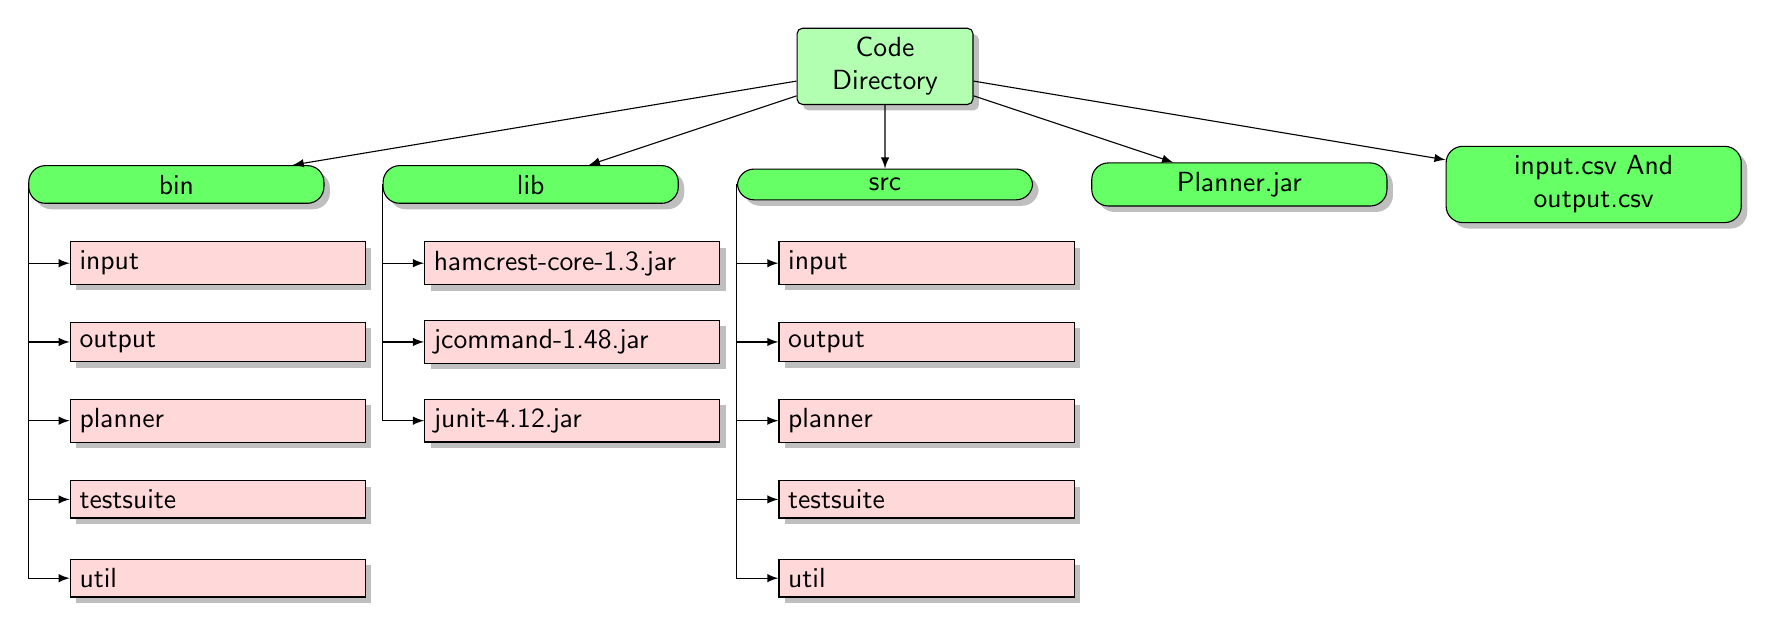
\begin{tikzpicture}[
  level 1/.style={sibling distance=45mm},
  edge from parent/.style={->,draw},
  >=latex]

% root of the the initial tree, level 1
\node[root] {Code Directory}
% The first level, as children of the initial tree
  child {node[level 2] (c1) {bin}}
  child {node[level 2] (c2) {lib}}
  child {node[level 2] (c3) {src}}
  child {node[level 2] (c4) {Planner.jar}}
  child {node[level 2] (c5) {input.csv And output.csv}};

% The second level, relatively positioned nodes
\begin{scope}[every node/.style={level 3}]
\node [below of = c1, xshift=15pt] (c11) {input};
\node [below of = c11] (c12) {output};
\node [below of = c12] (c13) {planner};
\node [below of = c13] (c14) {testsuite};
\node [below of = c14] (c15) {util};


\node [below of = c2, xshift=15pt] (c21) {hamcrest-core-1.3.jar};
\node [below of = c21] (c22) {jcommand-1.48.jar};
\node [below of = c22] (c23) {junit-4.12.jar};

\node [below of = c3, xshift=15pt] (c31) {input};
\node [below of = c31] (c32) {output};
\node [below of = c32] (c33) {planner};
\node [below of = c33] (c34) {testsuite};
\node [below of = c34] (c35) {util};

\end{scope}

% lines from each level 1 node to every one of its "children"
\foreach \value in {1,2,3,4,5}
  \draw[->] (c1.west) |- (c1\value.west);

\foreach \value in {1,2,3}
  \draw[->] (c2.west) |- (c2\value.west);

\foreach \value in {1,...,5}
  \draw[->] (c3.west) |- (c3\value.west);
\end{tikzpicture}
\end{landscape}
\end{document}
